\subsubsection{Leonardo Fibonacci e le scuole d'abaco.}\label{LeonardoFibonacciELeScuoleDAbaco}
\paragraph{Biografia di Leonardo Pisano, detto Fibonacci.} Poco \`e noto della vita di Leonardo Pisano. Egli nasce a Pisa verosimilmente tra il 1170 e il 1180 e in giovane et\`a segue suo padre, il mercante Guglielmo dei Bonacci, nella citt\`a di Bugia (odierna Algeria). Guglielmo \`e stato incaricato dal comune di Pisa di svolgere a Bugia le funzioni di \textit{publicus scriba pro pianis mercatoribus}, in un'epoca in cui Pisa, una delle famose repubbliche marinare, vanta un'importantissima presenza in tutto il Mediterraneo.
\par Guglielmo manda suo figlio Leonardo a studiare presso maestri arabi di matematica e il Fibonacci acquista le nuove conoscenze con grandissimo interesse, tanto da decidere di percorrere tutto il Mediterraneo alla ricerca di conoscenze aggiuntive: il risultato \`e l'opera pi\`u famosa di Fibonacci, l'enciclopedico \textit{Liber abaci} (1202), che descriveremo in dettaglio in seguito.
\par Il \textit{Liber abaci}, dopo poche iniziali difficolt\`a, si impone rapidamente come modello di manuale di aritmetica mercantile, tanto da portare alla fondazione di numerose scuole d'abaco, col preciso intento di insegnarne i contenuti. Leonardo stesso diventa maestro d'abaco, come dimostra chiaramente un documento datato del 1241 che lo assume presso il comune di Pisa con questa funzione.
\par Fibonacci scrive altre opere, tra cui la pi\`u importante \`e la \textit{Practica geometriae} (1220), un trattato di geometria da cui i maestri d'abaco traggono talvolta materiale per le loro lezioni. Intrattiene inoltre rapporti con Federico II di Svevia e la sua corte, tanto che molte delle sue opere sono dedicate a suoi membri. La data di morte \`e ignota.
\paragraph{Il \textit{Liber abaci}.} Il \textit{Liber abaci} \`e senza dubbio il pi\`u importante dei lavori di Fibonacci, prima di tutto per influenza. Il suo contenuto consiste in un'esposizione di tutta l'aritmetica araba sino circa ad Ab\=u K\=amil (circa 850 - circa 930), con l'importante influenza dei lavori di al-Khw\=arizm\={\i} (circa 780 - circa 850). Questa \`e la struttura del \textit{Liber abaci}:
\begin{itemize}
	\item capitoli 1-7: aritmetica -- cifre araboindiane, notazione posizionale, operazioni tra numeri interi e frazioni;
	\item capitoli 8-11: aritmetica mercantile -- cambi, pesi e misure, compravendita, baratti, distribuzione di profitti in societ\`a, fusione di monete;
	\item capitolo 12: curiosit\`a matematiche -- per esempio comprende la successione di Fibonacci derivata dal famoso problema dei conigli e il metodo della falsa posizione per la risoluzione di problemi che conducono a equazioni lineari del tipo $ax = b$;
	\item capitoli 13: il metodo della doppia falsa posizione per la risoluzione di problemi che conducono ad equazioni lineari del tipo $ax + b = c$;
	\item capitolo 14: estrazione di radici quadrate e cubiche;
	\item capitolo 15: proporzioni geometriche e algebra.
\end{itemize}
\par Lo stile dell'opera \`e retorico: il formalismo matematico \`e ancora molto rudimentale e si limita a fornire soluzioni sotto forma di ricette con un linguaggio pi\`u o meno uniforme.
\par Forniamo una breve descrizione della dimostrazione delle formule di risoluzione delle equazioni di secondo grado secondo gli arabi e dunque secondo Fibonacci. Innanzitutto, bisogna ricordare che la matematica araba non considera mai quantit\`a negative (neanche come soluzioni; anzi, spesso viene trascurata anche la soluzione nulla), pertanto le equazioni di secondo grado vengono per prima cosa classificate in forme normali, che riportiamo in notazioni moderne:
\begin{itemize}
	\item $ax^2 = bx$;
	\item $ax^2 = c$;
	\item $bx = c$;
	\item $ax^2 + c = bx$;
	\item $ax^2 + bx = c$;
	\item $ax^2 = bx + c$.
\end{itemize}
\par Le prime tre equazioni si risolvono facilmente con estrazioni di radici e metodo della falsa posizione. Le altre tre vengono ulteriormente normalizzate dividendo per $a$ (i \textit{censi}, cio\`e la quantit\`a di \textit{censi} cio\`e di quadrati dell'incognit\`a\footnote{L'incognita alla prima potenza si chiama invece \textit{radice} e la costante \textit{numero}; analogamente per \textit{radici} si intende la quantit\`a di radici dell'equazione, cio\`e $b$.}):
\begin{itemize}
	\item $x^2 + c = bx$;
	\item $x^2 + bx = c$;
	\item $x^2 = bx + c$.
\end{itemize}
\par Mostriamo come viene risolta la prima forma normale. Fibonacci, cos\`i come gli arabi, afferma che 
\begin{itemize}
	\item l'equazione \`e risolubile se e solo se $c \leq \left ( \frac{b}{2} \right )^2$, che equivale alla nostra ben nota condizione di risolubilit\`a;
	\item la soluzione, se esiste, \`e data da $x = \frac{b}{2} \pm \sqrt{ \left ( \frac{b}{2} \right )^2 - c}$.
\end{itemize}
\par La dimostrazione \`e geometrica. Proviamo che $x = \frac{b}{2} - \sqrt{ \left ( \frac{b}{2} \right )^2 - c}$ risolve l'equazione servendoci della figura \ref{Fibonacci_SecondoGrado}; la dimostrazione per l'altra radice \`e analoga. La nostra dimostrazione sar\`a generale, ma Fibonacci, che non ha ancora il simbolismo matematico moderno, prova le sue tesi attraverso esempi.
\begin{wrapfigure}{R}{0.5\textwidth}
	\includegraphics[width=0.48\textwidth]{Storia_della_matematica/Immagine_Fibonacci_SecondoGrado.png}
	\caption{Risoluzione dell'equazione di secondo grado secondo la quarta forma normale.}
	\label{Fibonacci_SecondoGrado}
\end{wrapfigure}
\par Il segmento $AB$ \`e lungo $b$ e $M$ ne \`e il punto medio. Sia il segmento $XB$ \`e uguale $x$ e supponiamo che $X$ giacia a destra di $M$\footnote{L'altro caso, quello in cui $X$ giace a sinistra di $M$, porta la seconda soluzione dell'equazione.}. Costruiamo il rettangolo $ABB'A'$ di base $AB$ e altezza $BB' = XB = x$ e il quadrato $XBB'X'$.
\par Ora, l'area del rettangolo $ABB'A'$ \`e $AB \cdot BB' = bx$, ma \`e anche $AX \cdot XX' + XB \cdot BB' = AX \cdot XX' + x^2$, da cui, poich\'e $x^2 + c = bx$, deve essere $c = AX \cdot XX'$.
\begin{wrapfigure}{R}{0.5\textwidth}
	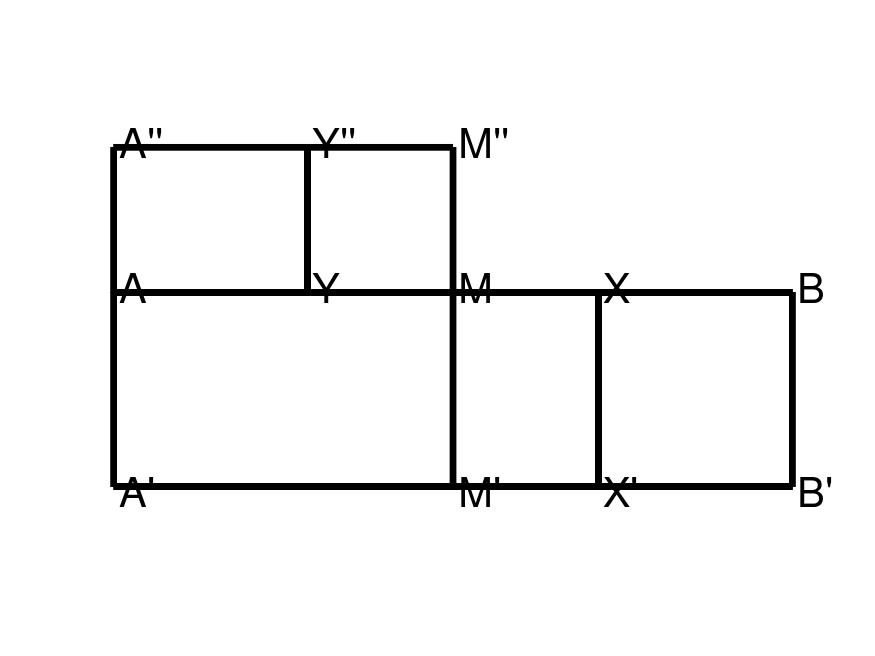
\includegraphics[width=0.48\textwidth]{Storia_della_matematica/Immagine_Fibonacci_SecondoGradobis.png}
	\caption{Risoluzione dell'equazione di secondo grado secondo la quarta forma normale, seconda parte.}
	\label{Fibonacci_SecondoGradobis}
\end{wrapfigure}
\par Costruiamo i quadrati $A'M'M''A''$ e $YMM''Y''$, dove $Y$ \`e il simmetrico di $X$ rispetto ad $M$. Allora il rettangolo $AYY''A''$ \`e congurente al rettangolo $MXX'M'$. Ne deduciamo che $AM^2 = AX \cdot XX' + MX^2$, da cui $\left ( \frac{b}{2} \right )^2 = c + MX^2$, da cui $x = MB - MX = \frac{b}{2} - \sqrt{ \left ( \frac{b}{2} \right )^2 - c}$ e questo conclude la dimostrazione.
\par La dimostrazione per l'altra radice \`e del tutto analoga e riportiamo solamente la figura (figura \ref{Fibonacci_SecondoGradoDue}; il segmento $AA'''$ \`e uguale a $AM$): lo stesso al-Khw\=arizm\={\i} non riporta la dimostrazione, ma le traduzione latine, come noi, riportano la figura. Il ragionamento cambia solo per la seconda parte in maniera immediata: $MX^2 = AM^2 - AX \cdot XX'' - X'''M''' \cdot M'''M'' = AM^2 - AX \cdot XX'' - A''X'' \cdot X''X' = AM^2 - AX \cdot XX' = \left ( \frac{b}{2} \right )^2 - c$.
\begin{wrapfigure}{R}{0.5\textwidth}
	\includegraphics[width=0.48\textwidth]{Storia_della_matematica/Immagine_Fibonacci_SecondoGradoDue.png}
	\caption{Risoluzione dell'equazione di secondo grado secondo la quarta forma normale, seconda radice.}
	\label{Fibonacci_SecondoGradoDue}
\end{wrapfigure}
\par Vediamo la seconda forma normale: in tal caso la soluzione \`e $\sqrt{c + \left ( \frac{b}{2} \right )^2} - \frac{b}{2}$. Abbiamo in questo caso due dimostrazioni geometriche.
\begin{wrapfigure}{R}{0.5\textwidth}
	\includegraphics[width=0.48\textwidth]{Storia_della_matematica/Immagine_Fibonacci_SecondoGrado2.png}
	\caption{Risoluzione dell'equazione di secondo grado secondo la quinta forma normale.}
	\label{Fibonacci_SecondoGrado2}
\end{wrapfigure}
\par La prima \`e illustrata dalla figura \ref{Fibonacci_SecondoGrado2}: si costruisce il quadrato di lato $x$ e sui suoi lati si costruiscono i rettangoli di altezza $\frac{b}{4}$. Allora l'area del quadrato di lati neri \`e $x^2 + 4 \cdot \frac{b}{4}x + 4 \cdot \left ( \frac{b}{4} \right )^2 = x^2 + bx + \left ( \frac{b}{2} \right )^2$. D'altra parte, essendo $x^2 + bx = c$, abbiamo che l'area del quadrato nero \`e $c + \left ( \frac{b}{2} \right )^2$. Se ne deduce che il lato del quadrato nero \`e $\sqrt{c + \left ( \frac{b}{2} \right )^2}$ e dunque il lato del quadrato blu $x = \sqrt{c + \left ( \frac{b}{2} \right )^2} - \frac{b}{2}$.
\par La seconda dimostrazione \`e del tutto analoga, ma invece di costruire quattro rettangoli rossi, ne costruisce solo due, su due lati perpendicolari del quadrato blu: aggiungendo il quadratino dell'angolo corrispondente del quadrato nero si ottiene un nuovo quadrato da cui si pu\`o partire per la nuova dimostrazione.
\begin{wrapfigure}{R}{0.5\textwidth}
	\includegraphics[width=0.48\textwidth]{Storia_della_matematica/Immagine_Fibonacci_SecondoGrado3.png}
	\caption{Risoluzione dell'equazione di secondo grado secondo la sesta forma normale.}
	\label{Fibonacci_SecondoGrado3}
\end{wrapfigure}
\par L'ultima forma canonica si risolve geometricamente con l'ausilio della figura \ref{Fibonacci_SecondoGrado3}: abbiamo $AB = x$, $AE = b$, $M$ punto medio di $FD$. I rettangoli rossi sono congruenti, dunque l'area del quadrato blu \`e uguale a quella del quadrato pi\`u piccolo ($\left ( \frac{b}{2} \right )^2$) pi\`u quella del rettangolo $CDEF$ ($(x - b)x = x^2 - bx = c$). Infine $x = AB = BM + MD = \frac{b}{2} + \sqrt{\left ( \frac{b}{2} \right )^2 + c}$, che \`e la soluzione.
\par Notiamo che negli ultimi due casi viene fornita una sola soluzione: ci\`o \`e coerente col fatto che la matematica allora non considerava mai le soluzioni negative, tradizione che durer\`a almeno sino a Descartes.
\par Il trattato \`e chiaramente rivolto ai mercanti, come si deduce subito dalla prevalente tipologia di problemi affrontati, e infatti gli stessi mercanti, dopo un'iniziale diffidenza verso i nuovi simboli rappresentati dalle cifre araboindiane, si convincono rapidamente della superiorit\`a dei metodi ivi esposti per la gestione dei propri affari, in un periodo storico in cui essi si trovano a gestire e registrare una gran quantit\`a di affari su vasta scala geografica. Non mancano dimostrazioni matematiche, come appunto le dimostrazioni geometriche delle formule fornite per risolvere le equazioni di secondo grado, sul modello di quelle di al-Khw\=arizm\={\i}, ma non esiste ancora, in quel periodo storico rimasto orfano della matematica greca, qualcuno che sia in grado di apprezzarle e ancor meno di migliorarle.
\par L'interesse pratico mercantesco e il disinteresse teorico porta alla fondazione delle scuole d'abaco.
\paragraph{Le scuole d'abaco.} Le scuole d'abaco, prodotto naturale del \textit{Liber abaci} pisano e degli interessi mercantili, si sviluppano naturalmente esclusivamente in Italia: un altro importante centro mercantile \`e quello delle Fiandre, ma la lontananza dal mondo arabo rende impossibile la comparsa di un lavoro simile a quello di Fibonacci e, non essendo ancora stata inventata la stampa, la diffusione dei testi \`e troppo ridotta per favorire uno scambio di conoscenze tra i due pi\`u grandi centri mercantili dell'epoca. Per gli stessi motivi, da notare il fatto che il maggior numero di scuola d'abaco sorge nei comuni maggiormente dediti al commercio e in Toscana: cos\`i una delle citt\`a con le migliori scuole d'abaco \`e inevitabilmente la citt\`a di Firenze, dedita al commercio e in Toscana.
\par Si stima che tra la fine del XIII secolo e la prima met\`a del XVI secolo vi erano circa 70 abacisti, quasi tutti maestri d'abaco, divisi in 20 scuole. Nel 1480, pi\`u del 25\% dei giovani istruiti avevan frequentato la scuola d'abaco; nel tardo Cinquecento, a Venezia, si raggiungeva il 40\%.
\par Le scuole possono essere private, pubbliche o anche finanziate parzialmente dal comune e parzialmente da chi le frequenta. Si entra alla scuola d'abaco circa all'et\`a di dieci anni e vi si resta per due, ma entrambi questi dati variano a seconda delle contingenze. Il programma \`e dato, di massima, dal contenuto del \textit{Liber abaci}, privilegiando i problemi di interesse mercantile, ma vi si potevano aggiungere elementi del \textit{Practica geometriae} o lezioni di grammatica, oltre naturalmente alla particolare esperienza del maestro. Come accennato, la matematica insegnata consiste in algoritmi di risoluzione ed esclude le dimostrazioni.
\par Nelle scuole d'abaco studiano grandi personalit\`a come Piero della Francesca e Leonardo da Vinci (1452-1519), i quali sono, oltre che due geni del rinascimento italiano, due esempi del fatto che tra gli studenti di queste scuole non vi sono solo mercanti, ma anche altre persone che si istruiscono fuori dalle universit\`a, dove dominano in lingua latina il diritto, la medicina, la teologia. Altro abacista di rilievo \`e senz'altro Niccol\`o Fontana (1499-1557), meglio conosciuto come Tartaglia, uno dei maggiori protagonisti del rinascimento matematico.
\par Come abbiamo cercato di spiegare, le scuola d'abaco rifondano il sapere matematico, su basi quasi estranee alla matematica greca antica, ma non solo: lo sviluppano anche. In particolare, per esempio, Piero della Francesca tenta di fondare matematicamente la prospettiva nel \textit{De prospectiva pingendi} (1475): l'influsso abacistico \`e evidente nell'impostazione, lontana dal metodo ipotetico deduttivo classico e strutturata in problemi da risolvere; altro esempio rilevante \`e quello dell'algebra, che si pone per la prima volta come la scienza che studia le equazioni a prescindere da qualsiasi applicazione concreta, anch'essa affrontata da Piero della Francesca che tenta di fornire soluzioni generali che funzionano per\`o solo per quelle equazioni che si presentano nel calcolo degli interessi composti: solo successivamente, grazie a Del Ferro (1465 - 1526), Tartaglia, Cardano (1501 - 1576), Ferrari (1522 - 1565) e anche Bombelli (1526 - 1572), che arriver\`a a tentare di introdurre i numeri complessi senza per\`o riuscirvi, si arriver\`a alle formule generali di risoluzione per le equazioni di terzo e quarto grado, con le limitazioni dell'epoca.
